\begin{frame}[fragile]{Some syntax}

\href{http://johnmacfarlane.net/pandoc/demo/example9/pandocs-markdown.html}{See
Pandoc markdown syntax here}

~

\emph{italics}

\textbf{bold}

\begin{verbatim}
verbatim
\end{verbatim}

No break paragraph like this.

But with 2 spaces\\at the end of the line.

vertical

~

space

\end{frame}

\begin{frame}{Slide with bullets}

\begin{itemize}
\itemsep1pt\parskip0pt\parsep0pt
\item
  one
\item
  two
\item
  three

  \begin{itemize}
  \itemsep1pt\parskip0pt\parsep0pt
  \item
    and a second level
  \item
    and more \ldots{}
  \end{itemize}
\end{itemize}

\begin{enumerate}
\def\labelenumi{\arabic{enumi}.}
\itemsep1pt\parskip0pt\parsep0pt
\item
  ONE
\item
  TWO
\item
  THREE
\end{enumerate}

\end{frame}

\begin{frame}[fragile]{Slide with subsections}

\begin{block}{Subsection one}

\begin{itemize}
\itemsep1pt\parskip0pt\parsep0pt
\item
  something here
\item
  more here
\end{itemize}

\end{block}

\begin{block}{Subsection two}

\begin{verbatim}
verbatim here
more
\end{verbatim}

\end{block}

\end{frame}

\begin{frame}{Slide with hyperlinks}

\url{http://ngscourse.github.io}

\href{https://github.com}{Follow the link}

\href{https://github.com}{Follow the link}

\begin{block}{Reusable Link}

\href{https://github.com/ngscourse/ngscourse.github.io/blob/master/README.md}{readme}

\href{https://github.com/ngscourse/ngscourse.github.io/blob/master/README.md}{Readme}

\href{https://github.com/ngscourse/ngscourse.github.io/blob/master/README.md}{README}

\href{https://github.com/ngscourse/ngscourse.github.io/blob/master/README.md}{go
to the readme}

\end{block}

\end{frame}

\begin{frame}{Big Image}

\begin{figure}[htbp]
\centering

\includegraphics[width=\textwidth,height=0.8\textheight,keepaspectratio]{images/smile}
\caption{caption here: do not use it}
\end{figure}

\end{frame}

\begin{frame}{Small Image (PNG)}

\begin{figure}[htbp]
\centering

\includegraphics[width=\textwidth,height=0.8\textheight,keepaspectratio]{images/small}
\end{figure}

\end{frame}

\begin{frame}{Square Image}

\begin{figure}[htbp]
\centering

\includegraphics[width=\textwidth,height=0.8\textheight,keepaspectratio]{images/square}
\end{figure}

\end{frame}

\begin{frame}{Horizontal image}

\begin{figure}[htbp]
\centering

\includegraphics[width=\textwidth,height=0.8\textheight,keepaspectratio]{images/horizontal}
\end{figure}

\end{frame}

\begin{frame}{Vertical image}

\begin{figure}[htbp]
\centering
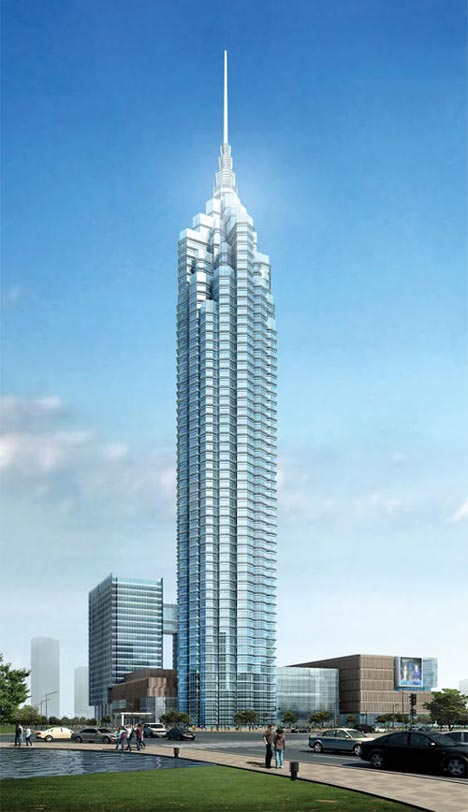
\includegraphics[width=\textwidth,height=0.8\textheight,keepaspectratio]{images/vertical}
\end{figure}

\end{frame}

\begin{frame}{SCALED image}

\centerline{
\includegraphics[scale=0.1]{images/smile}}

use \emph{proportions}

\end{frame}

\begin{frame}{Maths}

As in latex $X = Y$ inside the text

An equation:

\[f(x)=\sum_{n=0}^\infty\frac{f^{(n)}(a)}{n!}(x-a)^n\]

\end{frame}

\begin{frame}{Slide with two columns}

\begin{columns}\begin{column}{0.6\textwidth}\center

  Text and Images

  here

  But markdown is not working

  Hast to be \LaTeX

  - set relative sizes
  - of the columns 

\end{column}\begin{column}{0.4\textwidth}\center


\includegraphics[width=\textwidth,height=\textheight,keepaspectratio]{images/smile}

\end{column}\end{columns}

\end{frame}

\begin{frame}{Tables}

Not working at the moment

\end{frame}
